% Some commands used in this file
\newcommand{\product}{\textit}

\chapter{Material and Methods}

\section{General information}
All the liquids that will be in contact with the cell, are pre-warmed to limit cold-exposure. Unless specifically stated otherwise, we worked under sterile conditions. By courtesy of Dr. Ulrich Blache, we had access to human bone-marrow derived mesenchymal stem cells from anonymized patients with unknown medical history. Incubation parameters are kept constant at 37 \degC{} and 5\% CO2 in humidified air.

\section{Cell Culture And Passaging}

Cells are grown in growth medium under sterile conditions. Nunc\texttrademark{} EasYFlask\texttrademark{} Cell Culture Flasks with filters (ThermoFisher) were used for growing the cells. The media was changed every three days. Passaging was done at 80\% confluence using a standard TE-protocol. First, the cells are generously washed with PBS. Second, 2ml Trypsin-EDTA (TE, maduzi) is added, to detach the cells. After 5-10 minutes cells are round and detached as assessed by light microscopy. Then, add 10ml MEM\textalpha{} with 10\% FBS to deactivate the TE. Transfer cell solution to 15ml Falcon Tube and centrifuge for 5 minutes at a speed of 500 rcf. Next, discard the supernatant, leaving only the pellet. Resuspend the cells and seed according to application with typical seeding density being 10\textsuperscript{6} Cells / 75 cm\textsuperscript{2}. 
Growth Medium consist of ROTI\textregistered{} Cell Eagle's MEM-Alpha with nucleosides and stable l-glutamin(ROTH), 10\% FBS (heat-inactivated, Thermo Fisher) and 5ng/ml Growth Factor FGF-2 (PeproTech).

\section{Retroviral Transduction}
From 100\% confluent cells, seed cells at a ratio of 1:6 in T25 according to standard protocol. On the next day, remove medium, add 1ml of Polybrene-Medium (MEM\textalpha{}, 5\% FBS, 1\mul{}/ml Polybrene (Sigma-Aldrich)). From here onward, Biosafety Level (BL) 2 measures were applied. Carefully, add 1ml of virus construct to corresponding flask. Incubate at 4 \degC for two hours, followed by addition of 3ml Compensation-Medium (3ml MEM\textalpha{}, 5\% FBS, 1\mul{}/ml Polybrene and 8 ng/ml FGF-2). After letting it incubate at standard conditions overnight, remove medium and add 5ml standard growth medium. On the next day, split 1:3.5 depending on confluence. On the next day, start selection by removing old medium and adding Selection-Medium (Growth Medium + 3\textmu{}g/ml Puromycin) and incubating the cells for 72 hours. After incubation period has ended, pre-validate knock-out with comparing negative control (expected: low viability) to KO-cell-line (expected: high viability) under light microscope, similar to a smoke test. Over the next days, the cells are split another three times until the virus particles are \myworries{Word} and the Biosafety Level (BL) Restrictions can be relaxed from BL2 to BL1. Quality of knock-out is assessed with Western Blot (Protein) and qRT-PCR (mRNA). Freeze or cultivate according to need. 

\begin{figure}
    \centering
    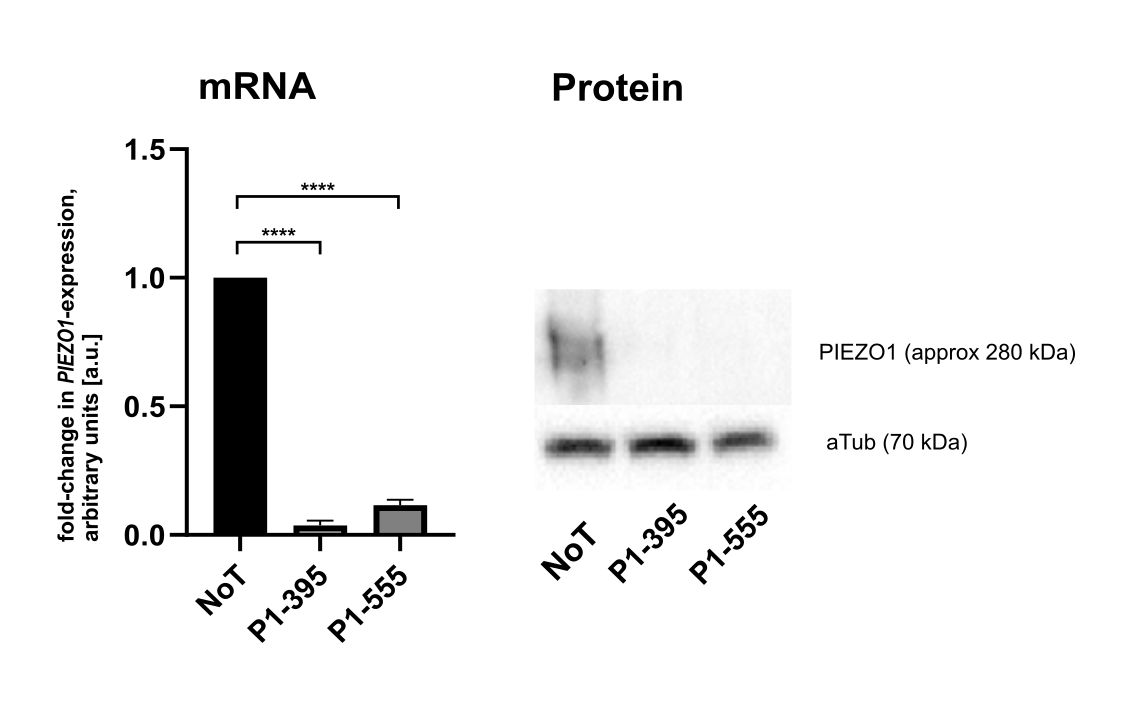
\includegraphics[width=\linewidth]{Piezo1KO_Verification_WBandPCR.png}
    \caption{Validation of successful knockout on mRNA (left) and Protein (right) level with housekeeping genes being RPL13A}
    \label{fig:KO-Verification}
\end{figure}

\section{RNA Analysis}
\subsection{RNA Extraction}
This was prepared in open space. Cells were either directly lysed in-well after PBS washing or lysed in the tube, after being collected from well and washed with PBS. Lysis-Buffer was supplemented with 1\% \textbeta-mercaptoethanol. The whole cell lysate was either frozen for later processing or directly processed. When freezing the lysate, the tube is shock-frozen in liquid nitrogen before transferred to -80 \degC freezer. When processing, the PureLink PCR Micro Kit (\product{Thermo Fisher, CN: K310250}) following manufacturer's protocol was used, dissolving the RNA in the final step with 20\mul{} of RNase-free Water (BioConcept). The final RNA concentration was measured using the Qubit RNA HS Assay Kit (ThermoFisher) with a new calibration each time a new working solution was prepared.

\subsection{Reverse Transcription}
This was prepared in open space. Unless stated otherwise, 300ng of RNA was transcribed per 40\mul{} total reaction volume using the High-Capacity cDNA Reverse Transcription Kit (Thermo Fischer) following supplier's instructions. \myworries{Insert program specification of Cindy Thermal Cycler (MasterCycler, Eppendorf)}. Samples were either stored at -20 \degC or immediately downstream processed. 

\subsection{Quantitative Real-Time PCR Analysis}
All real-time PCR analyses were performed on an StepOnePlus \myworries{CHECK THAT!} ThermoCycler real-time PCR system (Applied Biosystems) with a 96-well plate as a carrier device. Each reaction well contained a reaction volume of 2\mul{} sample cDNA and 8\mul{} Primer-specific PCR MasterMix (KAPA PROBE FAST MasterMix (KAPA Biosystems), TaqMan\textregistered{} Primer (ThermoFisher) and RNase-free Water(BioConcept)). The amplification protocol consisted of \myworries{CHECK THAT}. The C\textsubscript{t}-value (cycle threshold) value for each gene was determined using the automated threshold analysis in the StepOnePlus device. Data was evaluated using the comparative C\textsubscript{t}-Method with GAPDH and RPL13A as housekeeping genes.

Investigated gene products and corresponding primers used are: 
\begin{itemize}
\item COL1
\item COL3
\item FN1
\item IL6
\item IL11
\item ALPL
\item RUNX1
\item SPP1
\item GAPDH 
\item RPL13A
\end{itemize}

\section{Western Blots}
\subsection{Preparation}
After washing the cells with PBS, 0.5ml of TE(1X) was added to each well. Then, the cells are incubated for 3-8 minutes to allow for detachment. As to maximize yield, we additionally employed a scraping protocol. 1ml of MEM\textalpha{}+10\% FBS is added per well. Then with a cell scraper (Sarstedt) we scraped the cells and transferred the cell solution in a tube. This is followed by room-temperature centrifuge at 2'000 rcf for 5 minutes after which the supernatant is discarded. Then the tube is filled with 1.5ml of PBS and the centrifugation step including the discarding of supernatant. Finally, the tubes are shock-frozen in liquid nitrogen before transferring them to a -80 \degC freezer for storage.
When preparing the protein samples, 20\mul{} of \textsc{Ripa}-Buffer (Sigma-Aldrich) was added to the tubes containing the cell pellet in order to dissolve the pellet. After incubation on ice for 20 minutes, during which each sample was vortexed three to four times, the samples are 4 \degC centrifuged at maximum speed for 10 minutes. For further processing, only the supernatant is used. Measure protein concentration of all samples by employing the DC\texttrademark{} Protein Assay (BioRad), following the manufacturer's protocol and comparing it to the personal standard curve. Then protein concentration is normalized while maximized (i.e. dilute with RIPA all samples to match concentration of lowest concentration sample). 

\subsection{Western Blotting}
In new tube Laemmli-Buffer(6X) (BioRad) and sample was mixed to a final volume of 15\mul{}, then  vortex 5 seconds and then cooked for 4-8 minutes at 95 \degC in ThermoCycler (i.e. cooking). Then separate sample by SDS-PAGE (Used gel: 4–15\% Mini-PROTEAN TGX Stain-Free Protein Gel (BioRad) at constant current of 35 mA), then transferred onto PVDF Membrane (BioRad). The membrane was then blocked in 5 wt\% low fat dry-milk (Migros) in TBST (i.e. blocking solution) for 1 hour. This is followed by incubation primary antibody either for 2 hours at room temperature or 14 hours at 4 \degC{}. Then it is incubated in the matching secondary antibody, which is conjugated to HRP. Every time before immersion medium changes, the membrane was washed three times in TBST for 10 minutes. Either tUltra enhanced chemiluscence HRP substrate \myworries{Find this CN} has been used to produce a signal in machine \myworries{What machine}. Exposure time was manually adjusted to produce a representative picture of the samples at hand. Quantification was done manually with Fiji (version 2.0.0-rc-69, Java 1.8) following a slightly modified version of Luke Miller's method. [https://lukemiller.org/index.php/2010/11/analyzing-gels-and-western-blots-with-image-j/]

\begin{itemize}
    \item Primary Antibodies
    \begin{itemize}
        \item Col1a1
        \item aTub
        \item 
        \item 
    \end{itemize}
        \item Secondary Antibodies
    \begin{itemize}
        \item goat anti-mouse
        \item donkey anti-turkey
        \item 
        \item 
    \end{itemize}
\end{itemize}


\section{Chemical stimulation of \Piezo{} with \Yoda}
Experiment is initialised by employing a standard Trypsin-EDTA passaging protocol until after the centrifugation step. After centrifugation ended, the supernatant was discarded, the tube filled with 10ml sterile PBS, followed by another centrifugation step of 5 minutes at 500 rcf. Cell concentration was assessed right after transferring from Flask to Falcon Tube, using a Neubauer Improved Disposable Counting Chamber (\myworries{CHECKTHAT}). 
MSC were seeded in \myworries{CHECK PLATE} at a density of 240'000 Cells/4cm\textsuperscript{2} in serum-free MEM$\alpha$, without any addition of FGF-2. 4 wells per time-point, corresponding for each possible combination of  intervention and read-out method (Yoda/Control and Protein/RNA, respectively). This is followed by a resting period of 8-14h in the incubator to allow for cell attachment, before progressing with the intervention.
The intervention is initiated with a washing step, before 2.5ml of Intervention Medium (i.e. MEM\textalpha{} + 5\textmu{}M \Yoda (Sigma-Aldrich)) is added. Negative control samples were supplemented with MEM\textalpha{} only. The cells were then incubated for exactly 30 minutes, after which they are washed twice, before adding MEM\textalpha{} as culture medium. Harvesting of both RNA and Protein samples was done after 0, 24, 48 and 72hours using the standard protocol according to respective read-out method.\\ 

\section{Fluidic Shear Stress Model}
As the result of the Masters Thesis Project from Patrick Jäger, we have access to a device, a so-called flowchamber, that enables us to apply fluidic shear stress to cells in a fully controlled environment, with the only requirement of the cells being adherent. This flowchamber allows arbitrary choice of shear media, cell type and cellular alignment relative to flow, while leaving the researcher the opportunity to chose from either in-situ real-time calcium imaging, recultivation for additional steps or direct downstream processing.

\myworries{ADD FLOWCHAMBER PICTURE, Schematic from Eastbio Presentation}

\subsection{Flowchamber and seeding}
\label{sec:FluidicModel}

\myworries{Put a Picture of the flowchamber!}\\
To produce the PDMS part of the flowchamber, firstly, 10 parts of silicone \myworries{Product Name} and 1 part of cross-linker \myworries{Product Name} are combined and vigorously mixed for 5 minutes using a single-use spatula. Then put in vacuum chamber that oscillates between 60 and 120 mbar to rid the gel of all bubbles. Put the gel in negative, metal \myworries{form (?)}, then vacuum again. Then on heating plate \myworries{Manufacturer} over night at 70 \degC{}. After the microscopy slides underwent plasma treatment for 4 minutes, we glue a stamp on the slide using the silicon-crosslinker-mixture from earlier. Then we put them over night next to the metal form on a heating plate. On the next day, remove the PDMS-stamps, leaving behind PDMS grating. Decorate the stamps with Collagen-1 \myworries{Product Number} using Sulfo-SANPAH as a crosslinker. Separate the flowchamber pieces and punch entry point for syringe. Prepare glue by adding 3\mul of \myworries{Platinum Reagent} to 1g of silicon, mix for 3 minutes. Add 0.1g of Crosslinker, mix again for 5 minutes. Now glue PDMS-pieces on glass slide and put in oven at \myworries{40 deg C} for 2 hours. Either we stored them in the fridge or seed cells for an experiment on the next day.\\
For seeding, we work sterile in the cell culture lab. Flowchambers are sterilised through generous use of 80\% EtOH (including flushing of chamber). Flush the chamber twice with PBS. Prepare cell solution of 1 Mio Cells/ml in Growth Medium. Add 70 \mul{} of cell solution per flowchamber. After 45 minutes of incubation, flush the chamber with 200\mul{} of Growth Medium to remove non-adherent cells. Put in incubator over night with the experiment scheduled on the next day.

\subsection{Fluorescence staining and imaging}
In 500\mul{} of Growth Medium dissolve 2\mul{} Fluo-4 (ThermoFisher) (i.e. Staining Medium). Add 200\mul{} of staining medium per flowchamber and let it incubate 2h until the start of the experiment. 
Minimise photobleaching by decreasing unnecessary light exposition. In a dark microscopy room, connect the flowchamber with a syringe that is fixed on the NemeSys syringe system (Cetoni). The syringe holds artifical cerebrospinal fluid (ACSF),depending on the experiment mixed according to standard or calcium-free protocol, whose respective ingredients is described in the appendix \myworries{put that!}. The protocol used is stored in a \myworries{}. Imaging was done with excitation wavelength of \textlambda = 488 nm. Imaging protocol in LiveAcquisition (\myworries{versionNUMBER}, TILL Photonics) over 120 seconds per measurement incorporating a Z-stack of five layers to account for shear-mediated displacement of cell, which lead to a total of 600 pictures. Reduce image to one dimensional Z-projection with average intensity method.  \\
Note that in the extracellular Ca-influx experiment we flushed the flowchamber for 12 minutes (equivalent to 2.4ml medium) with normal ACSF in between measurements of the same cell patch.


\subsection{Processing and evaluation}

\begin{itemize}
\item n flowchambers per sample lead to pooled 3$\times$240 array, carrying [Mean, S(N), N]. No normalization between technical replicates with differing cell counts. 
\item One segmentation and normalisation per technical sample.
\item Processing pipeline with R and ImageJ. Custom scripts. One segmentation at the beginning of the first measurement, afterwards follow brightness of cell
\item An archived version of the macros used can be accessed on a link.
\item Maximum Values for peak-comparison were found by doing a maximum-search on the whole measurement interval. (Leading to maximum before stimulus in CaFree-measurements in some samples.)
\end{itemize} 


\section{Immuno-Staining and Confocal Microscopy}

